% This is a LaTeX thesis template for Monash University.
% to be used with Rmarkdown
% This template was produced by Rob Hyndman
% Version: 6 September 2016

\documentclass{monashthesis}

%%%%%%%%%%%%%%%%%%%%%%%%%%%%%%%%%%%%%%%%%%%%%%%%%%%%%%%%%%%%%%%
% Add any LaTeX packages and other preamble here if required
%%%%%%%%%%%%%%%%%%%%%%%%%%%%%%%%%%%%%%%%%%%%%%%%%%%%%%%%%%%%%%%

\author{Jeremy Forbes}
\title{What makes Australians vote the way they do?}
\degrees{B.Sc./B.Com., University of Monash}
\def\degreetitle{Econometrics Honours}
% Add subject and keywords below
\hypersetup{
     %pdfsubject={The Subject},
     %pdfkeywords={Some Keywords},
     pdfauthor={Jeremy Forbes},
     pdftitle={What makes Australians vote the way they do?},
     pdfproducer={Bookdown with LaTeX}
}


\bibliography{thesisrefs}

\usepackage{amsthm}
\newtheorem{theorem}{Theorem}[chapter]
\newtheorem{lemma}{Lemma}[chapter]
\theoremstyle{definition}
\newtheorem{definition}{Definition}[chapter]
\newtheorem{corollary}{Corollary}[chapter]
\newtheorem{proposition}{Proposition}[chapter]
\theoremstyle{definition}
\newtheorem{example}{Example}[chapter]
\theoremstyle{definition}
\newtheorem{exercise}{Exercise}[chapter]
\theoremstyle{remark}
\newtheorem*{remark}{Remark}
\newtheorem*{solution}{Solution}
\begin{document}

\pagenumbering{roman}

\titlepage

{\setstretch{1.2}\sf\tighttoc\doublespacing}

\chapter*{Preface}\label{preface}
\addcontentsline{toc}{chapter}{Preface}

This document is a research proposal, intended for submission as part of
the journey that is EBS Honours 2018.

The research proposed is an examination of the relationships that exist
between socio-demographics and voting behaviour in Australian federal
elections, and how this has changed over time. Considerations are The
data used in this study from every election and Census conducted since
2001.

\chapter{Introduction}\label{ch:intro}

Over the last two decades the Australian demographic profile has changed
significantly. An ageing population, higher levels of education across
the board, soaring house prices, the list goes on. At the same time, the
political landscape has been in a state of constant change, with the
country recently experiencing four leadership changes in just a five
year stretch. And yet the Australian support largely ebbs and flows
between the two major parties vying for power.

This leads to the question - why do Australians vote the way they do?

This research will explore the relationships that exist between
socio-demographics and voting behaviour in Australian federal elections,
and how this has changed over time, examining each election since 2001.

Socio-demographics are characteristics of a population, such as
percentage breakdowns by age, gender, ethnicity, education level and
income. The socio-demographic information used in this study is from the
Australian Census of Population and Housing, a country-wide survey
conducted every five years.

Federal elections on the other hand, are conducted every three years.

Utilising new tools in spatial analysis, this study aims to build
socio-demographic profiles for each electorate, at election time, using
the available Census information. On reviewing the literature, it
appears that the approach of imputing electorate profiles that is
proposed in this study is a new innovation in socio-political analysis.

At the centre of this study are three key questions:

\begin{enumerate}
\def\labelenumi{\arabic{enumi}.}
\item
  What are the demographic factors that affect preference between the
  two major parties?
\item
  What factors are linked with electorate support for the full political
  spectrum?
\item
  How have these changed over time?
\end{enumerate}

There are three ways in which this research differs from other voting
studies. Firstly, it uses spatial modelling tools to impute
socio-demographic information for an election, using Census information
from nearby years. Secondly, it considers predictive modelling for
electorate voting behaviour, and thirdly it combines information for
every election since 2001.

\section{Data sources and mapping}\label{data-sources-and-mapping}

In order to impute socio-demographics at election time, the algorithm
proposed in this research follows the dominant approach in spatial
studies by overlaying maps that are in Geographic Information Software
(GIS) format. Overlaying GIS maps is used in other analyses of
Australian voting behaviour, and other fields including; strategic
planning \autocite{Valcik12}, healthcare \autocite{Ye17} and
geosciences. Maps are collected from the Australian Bureau of Statistics
and the Australian Electoral Commission.

\section{Modelling}\label{modelling}

Answering question (1) involves modelling the preference between the two
major political parties as a function of an electorate's
socio-demographics. The vote for one of these parties, \(TPP_i\), sits
in the interval \([0,1]\), and can be modelled using a logistic
transform, so that it maps on \(\mathbb{R}\).

Question (2) involves modelling the votes for multiple groups. The votes
for each party in an electorate can be treated as a proportion of the
total votes for that electorate. Denoting \(FP_i\) as the proportion of
vote for party \(i\), then \(\sum_{i=1}^D FP_i = 1\), for \(D\) parties,
making this a compositional dataset. Candidate approaches for modelling
include the Dirichlet distribution and logratio transformations of the
data.

Observing how these relationships change over time will be embedded in
the models addressing questions (1) and (2).

\section{Reproducible and openly
available}\label{reproducible-and-openly-available}

All content produced in this study reproducible and data used is
publicly available, so this project provides a resource for future
research. A key deliverable is the contribution made to the \(eechidna\)
R package, which includes the GIS maps, data from both all censuses and
elections, and the imputed socio-demographic electorate profiles at the
time of each election. When the next elections and Censuses come around,
the \(eechidna\) package will provide a resource for anyone to conduct
their own socio-political analysis. The name \(eechidna\) is an acronym
for `Exploring Election and Census Highly Informative Data Nationally
for Australia'.

\chapter{Literature Review}\label{ch:litreview}

\section{Spatial analysis of Australian
elections}\label{spatial-analysis-of-australian-elections}

Existing spatial analyses of Australian elections appear to focus on a
single federal election, with socio-demographic information pulled from
the nearest census. This approach is used in \textcite{Stim06}, and is
adapted to an online e-research platform by \textcite{Liao09}. Both use
GIS to connect Census and election data. However, both Stimson et al.
and Liao et al. use information disaggregated to polling booth locations
- a greater level of disaggregation than electorates, which the grouping
of focus of this study.

Seemingly vacant in Australian studies is the examination of these
socio-political relationships over time. It appears that no study has
either attempted to create a collection of socio-demographics for
multiple elections, or connect information from multiple censuses to a
single election - an approach that will be explored for the election
years in which a Census does not fall.

A popular approach in single-election studies is to focus analysis on a
single electoral division \autocite{Forrest01}, or a particular
political party \autocite{Davis98}. \textcite{Stim12} expand on this by
modelling relationships between population variables and voter support
for political parties, using univariate visualisations, linear
regressions, summary statistics and discriminant analysis. Discriminant
analysis is also used by \textcite{Stim06} because it aims to
distinguish between political parties in their voter support, rather
than predict how areas would vote.

\section{Modelling with compositional
data}\label{modelling-with-compositional-data}

In order to answer research questions (1) and (2), this study focuses on
regression models for inference and prediction. Response variables for
these questions are non-negative and sum to unit, making them
compositional with \(D\) components \autocite{PG11}.

The two popular approaches to modelling compositional data are by way of
logratio analysis, and the Dirichlet distribution.

Logratio analysis \autocite{JA86} uses a transformation of the
components, which then can be treated as a multivariate distribution.
Available transformation methods are additive, centred and isometric
\autocite{Ego03}. A common method is to treat the transformed data as
multivariate normal, which allows for covariation between the parts. In
modelling the 2001 Australian federal election, \textcite{Chong05} adopt
this technique, using an additive logratio transformation.

The Dirichlet distribution also provides a candidate for modelling the
distribution of votes, as the components estimated must sum to one.
\textcite{Campbell87} propose a covariate extension which allows for
parameters to be functions of covariates. This approach is adopted by
\textcite{Gueor08} in estimating component scores of a psychiatric
assessment, with parametric regression used to estimate the Dirichlet
parameters.

\chapter{Data}\label{ch:Data}

The two main data sources for this research are the Australian Census of
Population and Housing from the Australian Bureau of Statistics (ABS),
and published federal election results from the Australian Electoral
Commission (AEC).

The Census of Population and Housing collects data on the key
characteristics of every Australian, and is conducted every five years.
There have been four censuses in the 21st century, being that in 2001,
2006, 2011 and 2016. The information contained in these collections are
used to build the socio-demographic profiles for each electorate.

Federal elections typically occur every three years, and the those of
interest are the 2001, 2004, 2007, 2010, 2013 and 2016 elections. All
information from these sources are publicly available.

\section{Electorates and their
boundaries}\label{electorates-and-their-boundaries}

Australian Federal elections are determined based on which party wins a
majority of the 150 seats in the House of Representatives, with each
seat corresponding to an electorate. The electorate boundaries are
determined by population, and to ensure equal representation, the
boundaries of these divisions have to be redrawn regularly by the AEC.
Each redistribution typically affects a handful of electorates, with
most remaining the same as previously defined.

Since changes are continually made to electoral boundaries, when it is
time for a Census to be conducted, the ABS constructs an approximation
to the current electorates and aggregates data at this level.

What this means is that the electorate boundaries in the election prior
to a Census may not match the boundaries used in the Census, which may
not match the boundaries in the following election and so on.

This presents a challenge. How does one construct socio-demographic
profiles at election time for each electorate, when we cannot directly
match that election with a censuses?

\section{Census}\label{census}

\subsection{Collection}\label{collection}

Data for each Census are downloaded as a collection of Microsoft Excel
spreadsheets, with each spreadsheet corresponding to a particular
electorate, or a particular question (depending on the format used in
that Census year).

In order to convert the information held in these spreadsheets into a
summarised table containing selected socio-demographics for each
electorate, a series of \(R\) scripts and \(R{\text -}markdown\) files
have been created. The output of each file is an \(R\) data.frame
object, which tabulates the selected metrics for that Census year.

There was no way to automate this process, and the formats of each
Census collection change slightly each year. As such, it has taken a
significant amount of time and effort to extract the information from
excel, and wrangle the data into the desired metrics and format. A
snippet of the raw data can be found in the appendix
\ref{fig:excel-demo}.

The resultant data.frame for each election contains information for each
electorate on:

\begin{itemize}
\item
  State
\item
  Population
\item
  Age
\item
  Education
\item
  Employment
\item
  Religious and cultural identity
\item
  Median incomes (personal, household, family)
\item
  Median rent and loan payments
\item
  Citizenship and birthplace
\item
  Language at home
\item
  Relationship status
\end{itemize}

All metrics are recorded as percentages, representing the percentage of
people in that electorate who satisfy the category in question. For
example, \(AusCitizen\) is the percentage of people in the electorate
who are Australian citizens.

A full description of socio-demographic variables in the electorate
profiles can be found in the appendix \ref{ch:appendix}.

\subsection{Insights on the changing Australian
demographic}\label{insights-on-the-changing-australian-demographic}

Comparing Census data across years reveals many insights into how the
Australian demographic has changed over the past 17 years. By examining
visual distributions of metrics across Census years, trends can be
identified for the entire country and for the spread amongst
electorates.

\subsubsection{As Australians grow old, some stay
young}\label{as-australians-grow-old-some-stay-young}

It is well documented that Australia has an ageing population, and this
is reflected in the MedianAge plot {[}\ref{fig:vis-age}{]}, as we see
the distribution of median age across electorates spread upwards, with
some electorates in 2016 having a median age of 50 years old. However,
some electorates are not ageing as others do, which makes intuitive
sense, because some areas may be more suitable for particular age
brackets.

This is exactly the effect we see in young adults. Those aged 25-34 are
more likely to congregate in common electorates, and avoid other
electorates than they were in 2001 - making up 35\% of the population in
some electorates.

\begin{figure}
\centering
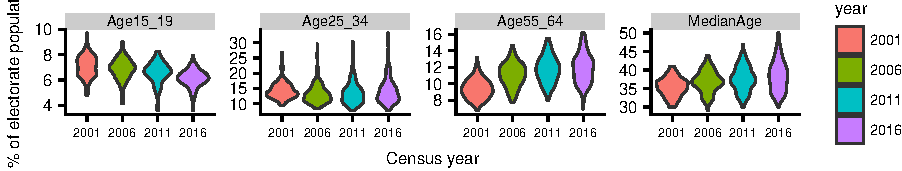
\includegraphics{thesis_files/figure-latex/vis-age-1.pdf}
\caption{\label{fig:vis-age}Age profile of Australian electorates}
\end{figure}

\subsubsection{Religion - a thing of the
past?}\label{religion---a-thing-of-the-past}

Socially ``progressive'' movements continue to gather momentum all over
the world, and as a result, Australia is moving away from traditional
religious beliefs and values. The frequency of individuals not
identifying with a religion has grown significantly over the years. This
effect has stretched across (what appears to be) every electorate
{[}\ref{fig:vis-relig}{]}. Having a religious identity of any kind would
make you a minority in some electorates! At the same time, particular
electorates maintain large representation of a particular religious
group, as seen by thin upper tails of the Buddhism, Islam and Judaism
metrics.

\begin{figure}
\centering
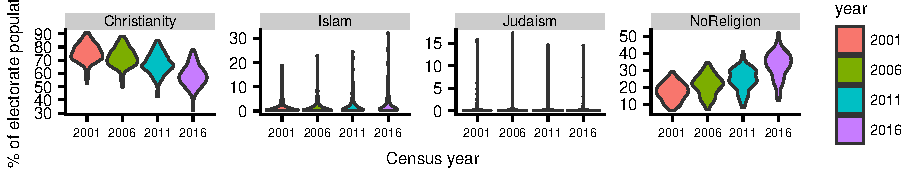
\includegraphics{thesis_files/figure-latex/vis-relig-1.pdf}
\caption{\label{fig:vis-relig}Religious profile of Australian electorates}
\end{figure}

\subsubsection{Investing in education}\label{investing-in-education}

Australia has seen improvements in education outcomes across the board,
experiencing continual increases in secondary and tertiary competion
rates across the years {[}\ref{fig:vis-educ}{]}. It is encouraging to
see that no electorates appear to be lagging behind, as the minimum
values increase each year for all levels of education.

\begin{figure}
\centering
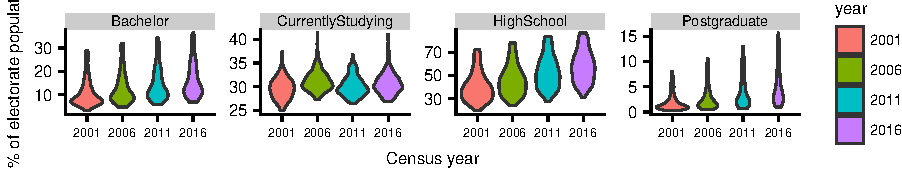
\includegraphics{thesis_files/figure-latex/vis-educ-1.pdf}
\caption{\label{fig:vis-educ}Education profile of Australian electorates}
\end{figure}

Violin plots of the complete set of variables in the electorate profiles
can be found in the appendix, see \ref{fig:vis-census}.

\paragraph{A note on Census
non-response}\label{a-note-on-census-non-response}

Like in any survey, non-response bias is a source of potential problems.
ABS statements released with each Census assure a high quality of data
collection, and this study assumes its reliability.

Non-response for key variables is imputed by the ABS (age, sex, martial
status and usual residence) for 2006, 2011 and 2016, although is not
clear whether this has been done in 2001. Non imputed items are treated
as ``not stated'' or ``not applicable'', dependent on the imputed age of
the person.

No adjustments or imputations are made in this study to the values
derived from each Census. However, the frequency of ``not stated''
responses will be recorded for particular questions, and are included
with other Census-derived metrics in the electorate profiles.

\section{Elections}\label{elections}

Within each electorate, candidates from various political parties will
run for election to represent that electorate. Voting is compulsory in
Australia, and the winning candidate is determined by preferential
voting. This means that each person assigns a numbered preference to
each candidate, and the winner is determined by receiving a majority of
preference votes.

At the end of tallying the first round of preferences, if there is no
majority, the party with the least votes will have its first preference
vote distributed to the parties that voters had selected as their second
preference. This is continued until a party receives an absolute
majority of votes.

The three type of vote counts are published for each federal election,
they are as follows.

\begin{itemize}
\item
  Division of preferences: distribution of preferences at each step of
  reallocation, beginning with first preferences.
\item
  Two party preferred: distribution of preferences where, by convention,
  comparisons are made between the ALP and the leading Liberal/National
  candidates.
\item
  Two candidate preffered: distribution of preferences to the two
  candidates who came first and second in the election.
\end{itemize}

For this study, the two party preferred and division of preferences
outcomes are used to answer research questions (1), (2) and (3).

These can be downloaded directly from the AEC website, and have been
compiled and stored in \(R\) data.frames, using the same method as
described for the Census data.

\section{Mapping socio-demographic profiles to election
times}\label{mapping-socio-demographic-profiles-to-election-times}

The elections and censuses have different frequencies, occuring every
three and five years respectively. This naturally leads to a significant
challenge in conducting socio-political analysis over time,
mapping\ldots{}

\begin{itemize}
\item
  A Census to an election that fall on the same year
\item
  Census information to an election that does not fall on a Census year
\end{itemize}

\begin{figure}

{\centering 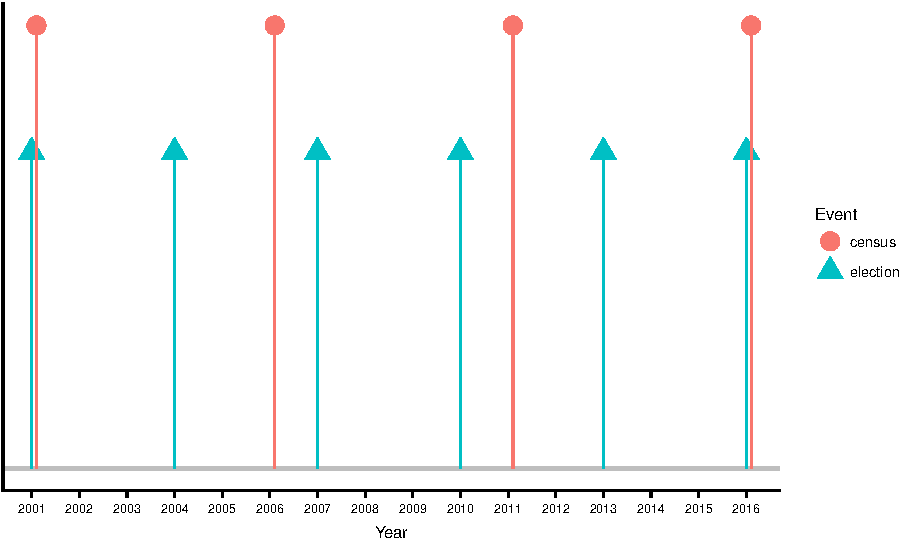
\includegraphics[height=0.3\textheight]{thesis_files/figure-latex/unnamed-chunk-1-1} 

}

\caption{Timeline of Australian elections and censuses}\label{fig:unnamed-chunk-1}
\end{figure}

\subsection{Elections that fall on a Census
year}\label{elections-that-fall-on-a-census-year}

When a Census is conducted in an election year the electorate boundaries
used by the ABS match the AEC electoral divisions for that election, so
the Census profiles for each electorate can be directly mapped to the
election time. This is done by joining information from the 2001 and
2016 data.frames.

\subsection{Elections that do not fall on a Census
year}\label{elections-that-do-not-fall-on-a-census-year}

If the election does not fall on the same year a Census is conducted,
two problems arise:

\begin{itemize}
\item
  Electorate boundaries may not match any of the neighbouring censuses
\item
  Demographics may have changed since the last Census was conducted
\end{itemize}

This study proposes an innovative projection algorithm using GIS maps,
\(k{\text -}centroid \space mapping\), for imputing the demographic
profiles for each election, accounting for both the time of the election
and the boundaries in place. The use of GIS maps to overlay data from
multiple sources is a dominant approach in spatial studies, which
provides the foundation for \(k{\text -}centroid \space mapping\).

\section{K-centroid mapping}\label{k-centroid-mapping}

For the purpose of illustrating the algorithm, ``division'' will be used
instead of ``electorate''.

\(k{\text-} centroid \space mapping\) is a method of imputing Census
demographics for divisions in place at the time of an election. Using
tools predominantly from the \(rgeos\) package, each boundary at
election time is superimposed on top of the divisions at a particular
Census time to determine which of the Census divisions intersect with
the superimposed boundary. For each division that intersects the
boundary, its area of intersection with the superimposed boundary is
computed. These areas are used to impute the composition of the
population that sit within the election boundary, where each person is
categorised by their Census division. A weighted average of demographics
from the Census divisions is then used to impute the socio-demographic
profile of the election boundary. This is done for each of the election
divisions, and the process repeats for the other Census. Interpolating
between the two censuses, based on time, yields the final imputed
profiles.

The \(k{\text -}centroid \space mapping\) algorithm for imputing the
socio-demographic profiles for divisions defined at the time of an
election is as follows:

\begin{enumerate}
\def\labelenumi{\arabic{enumi}.}
\tightlist
\item
  Select the nearest censuses that occur before and after election time.
\end{enumerate}

To map the 2013 Federal election profiles, we would select the censuses
from 2011 and 2016.

\begin{enumerate}
\def\labelenumi{\arabic{enumi}.}
\setcounter{enumi}{1}
\tightlist
\item
  Simplify the GIS maps for the division boundaries for each Census, and
  the election.
\end{enumerate}

Using \(gSimplify\) from the \(rgeos\) package, we reduce the size of
the maps (by reducing the number of points) to reduce computational
burden. This step is not necessary but helps the processing of large
maps.

\begin{enumerate}
\def\labelenumi{\arabic{enumi}.}
\setcounter{enumi}{2}
\tightlist
\item
  For each map, calculate the centroid of each division.
\end{enumerate}

Centroids for each polygon (division) are defined as using Euclidean
distance.

\begin{enumerate}
\def\labelenumi{\arabic{enumi}.}
\setcounter{enumi}{3}
\tightlist
\item
  Select an election division and create a map containing Census
  divisions with \(k\) closest centroids to the election division.
\end{enumerate}

Now consider only the division ``Brisbane'' in the 2013 election. The
polygon for its boundaries is shown in \ref{fig:bris-k3} by the dotted
blue line, with the boundaries of the closest \(k = 3\) divisions at the
time of the 2011 Census shown in red.

Note: \(k = 3\) is chosen here to illustrate how the algorithm
functions. The selection of \(k\) depends on the properties of the two
maps. We see here that \(k = 3\) is a sufficient choice, because there
do not appear to be parts of the 2013 division that sit outside of the 3
nearest divisions, but this may not be the case for other 2013
divisions. For this study, \(k=35\) is chosen due to the variation in
sizes of the divisions, as a neighbouring division can be very large and
have a distant centroid.

\begin{figure}

{\centering 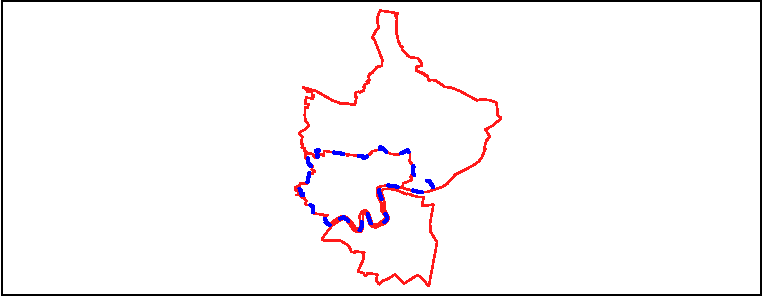
\includegraphics[width=0.7\linewidth]{thesis_files/figure-latex/bris-k3-1} 

}

\caption{Brisbane and the k=3 closest divisions}\label{fig:bris-k3}
\end{figure}

\begin{verbatim}
## integer(0)
\end{verbatim}

\begin{enumerate}
\def\labelenumi{\arabic{enumi}.}
\setcounter{enumi}{4}
\tightlist
\item
  For each of the \(k\) closest Census divisions, determine the area of
  intersection with the election division.
\end{enumerate}

Continuing with Brisbane from 2013, we see the area of overlap each of
Brisbane, Griffith and Lilley from the 2011 boundaries, given by the
shaded blue region {[}\ref{fig:bris-ints}{]}.

In general, this would be done between the Brisbane (2013) and every one
of its \(k\) nearest 2011 divisions.

\begin{figure}

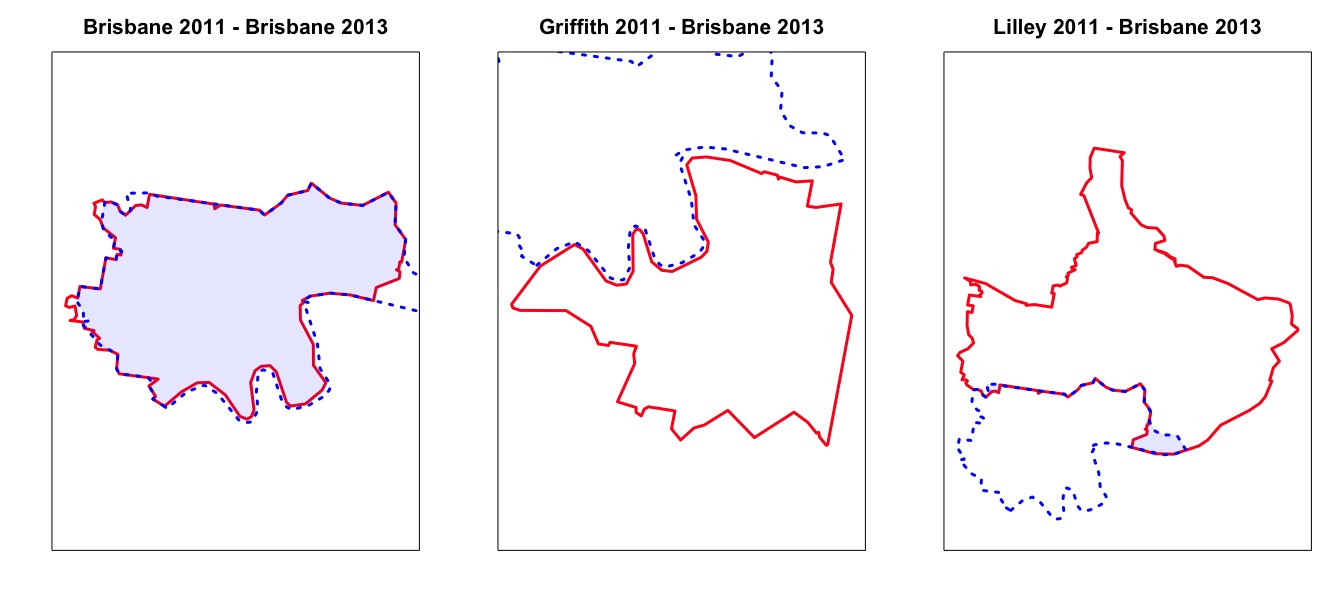
\includegraphics[width=1\linewidth,height=0.28\textheight]{/Users/Jeremy/Documents/R/MonashThesis-master-DONOTEDIT/data/Brisbane-Intersect} \hfill{}

\caption{Intersection of Brisbane (2013) and nearby Census divisions (2011)}\label{fig:bris-ints}
\end{figure}

\begin{enumerate}
\def\labelenumi{\arabic{enumi}.}
\setcounter{enumi}{5}
\tightlist
\item
  Calculate the number of people each intersect represents.
\end{enumerate}

We see that the shaded intersection areas are only a piece of their 2011
Census division. The population of Lilley (2011) is \(145,652\), and the
intersection with Brisbane (2013) is approximately \(2.22\%\) of the
total area in Lilley, so the population captured by the shaded area is
\(3,233\). Here we assume population is equally spread throughout each
division.

\[PopulationInt_{Lill} = \frac{Area_{intersect}}{Area_{Lill}} \cdot Population_{Lill} = 0.222 \cdot 145,652 \approx 3233\]

The intersection of Brisbane and Brisbane equates to 99.00\% of the 2011
Brisbane division. Brisbane (2011) has a population of \(145,051\), so
intersection represents approximately \(143,602\) people. There is no
overlap with Griffith (2011).

\begin{enumerate}
\def\labelenumi{\arabic{enumi}.}
\setcounter{enumi}{6}
\tightlist
\item
  Determine the socio-demographic profile based on the people in each
  intersection, where each person assumes the demographic composition of
  their Census division.
\end{enumerate}

Brisbane (election, 2013) is made up of \(143,602\) people from Brisbane
(Census, 2011) and \(3,233\) people from Lilley (Census, 2011). To
impute each socio-demographic statistic for the Brisbane division
(2013), we take a weighted average of the Census demographics, using the
intersection populations, \(PopulationInt\), used as the weights.

For example, estimating \(AusCitizen\) for the superimposed Brisbane
(2013) election boundary is done by a weighted average of its
intersection with Lilley and Brisbane.
\[\hat{AusCitizen_{Bris,Election}} = \frac{AusCitizen_{Bris,Census} \cdot PopulationInt_{Bris} + AusCitizen_{Lill,Census} \cdot PopulationInt_{Lill}}{PopulationInt_{Bris} + PopulationInt_{Lill}}\]

\begin{enumerate}
\def\labelenumi{\arabic{enumi}.}
\setcounter{enumi}{7}
\item
  Repeat steps 4-7 for each election division.
\item
  Interpolate between the Censuses by year to impute the
  socio-demographic division profile for the election year.
\end{enumerate}

The 2013 election sits two years after the 2011 Census, and three years
before the 2016 Census. Take a weighted average of each demographic
across time points for each division.
\[\hat{AusCitizen_{Bris,Election,2013}} = \frac{2}{5} \cdot \hat{AusCitizen_{Bris,Election,2011}} + \frac{3}{5} \cdot \hat{AusCitizen_{Bris,Election,2016}}\]

\chapter{Modelling \{ch: Modelling\}}\label{modelling-ch-modelling}

Now that estimated socio-demographic profiles have been obtained for
each election, we begin modelling to answer the questions that were set
out in the introduction:

\begin{enumerate}
\def\labelenumi{\arabic{enumi}.}
\item
  What are the demographic factors that affect preference between the
  two major parties?
\item
  What factors are linked with electorate support for the full political
  spectrum?
\item
  How have these changed over time?
\end{enumerate}

\section{Major party preference}\label{major-party-preference}

Question (1) is concerned with modelling the two party preferred vote,
\(TPP\), to analyse preference between Labor and Liberal/National
parties. Since \(TPP_{Labor} + TPP_{Liberal} = 1\), we can focus our
models on the response \(TPP_Labor\), which sits in the interval
\((0,1)\). This can be modelled using a logistic normal distribution:

\[f(TPP) = \frac{1}{\sigma \sqrt{2 \pi}} \frac{1}{TPP(1-TPP)}\exp(-\frac{(logit(TPP)-\mu)^2}{2\sigma^2})\]

where \(logit(TPP)\) is the logistic transformation
\(ln(\frac{TPP}{1-TPP})\).

The mean \(\mu\) is a parametric function of the socio-demographics
\(\bf X\) of each electorate \(\mu = f({\bf x})\). We can then use basic
regression techniques to estimate the regression coefficients, by way of
the \(lm()\) function.

Inference can then be conducted on the output, in order to determine
which factors are statistically significant, and their marginal effects
on the two party preferred vote.

\section{The full spectrum}\label{the-full-spectrum}

In order to model support for all parties, the first preference
allocation from the division of prefences is used. Let
\(\textbf{v}_i = (v_{i1}, v_{i2}, ..., v_{iD})\) denote the vector
holding the percentage of first preference votes for parties in
electorate \(i\), for each of the \(D\) parties. This presents an
extension to the modelling for the two party preferred vote.

The two party preferred vote has \(D=2\) parties, so the data is
compositional with \(D=2\) components. First preference vote has \(D>2\)
for every electorate in each election, and we still have
\(\sum_{j=1}^Dv_{ij} = 1\), so we have to consider other avenues for
modelling.

Two candidate methods for modelling first preferences are:

\begin{itemize}
\item
  Logratio analysis
\item
  Dirichlet covariate modelling
\end{itemize}

Both methods will be used to produce models for first preference, and I
will draw conclusions based on the consistency of effect that
socio-demographics across models.

\subsection{Logratio analysis}\label{logratio-analysis}

Logratio analysis (Aitchison 1986) uses the transformation of the
response \(\textbf{v}_i\) to \(\textbf{w}_i\), where
\(\textbf{w}_i \in \mathbb{R}^D\) (or \(\mathbb{R}^{D-1}\)), so
\(\dim(\textbf{w}_i) \text{ is } D\times1 \text{ or } (D-1) \times 1\),
depending on the transformation method. To obtain
\(\textbf{w} = (w_{i1}, w_{i2}, ..., w_{iD})\) or
\(\textbf{w} = (w_{i1}, w_{i2}, ..., w_{i(D-1)})\) there are three
available mappings: additive, centred and isometric. Each of these
mapping techniques will be tested to see which performs best, and which
is easily interpretable.

Note that the \(D=2\) case using the additive transformation is the same
as doing a logistic transform, so answering question (1) is following
the same method.

The transformed \(\textbf{w}_i\) can be modelled as multivariate normal,
\(\textbf{w}_i \sim{N({\mu_i}, {\bf \Sigma}})\), where each component
has a different mean modelled as a function of socio-demographics,
\({\bf\mu}_i = f({\bf x}_i)\). Parametric specifications of
\(f({\bf x}_i)\) will be used. Further investigation is required into a
suitable functions for estimating the coefficients in \(f({\bf x}_i)\)
and \({\bf \Sigma}\).

More on the three transformation methods can be found in the appendix
\ref{ch:appendix}.

\subsection{Dirichlet covariate
modelling}\label{dirichlet-covariate-modelling}

A modified version of the Dirichlet distribution \autocite{Campbell87}
provides another method of modelling the vector of first preferences.
This version, called the Dirichlet covariate model, the parameters of
the Dirichlet distribution can be estimated as a function of covariates,
\(\lambda_j = h_j({\bf x})\).

Dirichlet regression can be done in \(R\) using the \(DirichReg\)
package, and parametric forms of \(h({\bf x})\) will be chosen.

\section{Change over time}\label{change-over-time}

This is an area that requires some more thought. Current plans are to
estimate models for each of the elections separately, and examine how
the influence of factors differ across models.

An extension would be to track electorates over time - however this is
tricky since electorate boundaries are changing across elections. It may
be possible to gather votes from a different level of aggregation, like
polling booths, and use a similar technique to
\(k{\text -}centroid \space mapping\) to create voting statistics for
each election, based on the 2016 boundaries.

\section{Model Assessment and
Diagnostics}\label{model-assessment-and-diagnostics}

Tests for high leverage and goodness of fit will be done for each
category of models, as will model selection within each category.

High leverage will determine whether particular electorates are outliers
from the rest, in terms of the relationship between socio-demographics
and voting behaviour. Common tests for high leverage to be conducted
will include Cook's distance and Likelihood distance \autocite{RC82}.

Goodness of fit tests will determine how well the data fits the imposed
model structure. Tests will include Pearson's Chi-Square and Aitchison's
\({\text R}^2\) measure of total variability \autocite{JA86}.

Comparative model assessment criteria will include Aikaike Information
Criteria (AIC) and the Likelihood-ratio test, in order to determine the
best models from each category.

\chapter{A brief reflection and discussion \{\#ch:Reflection \&
Discussion\}}\label{a-brief-reflection-and-discussion-chreflection-discussion}

To date, all effort has been directed towards gathering, cleaning and
wrangling the data from the ABS and AEC into workable \(R\) objects.
Navigating the AEC and ABS websites to obtain the vote counts and Census
data was relatively straightforward, although the 2001 election required
direct contact with the AEC, as it is not downloadable online. Finding
the GIS maps for each event was a little more difficult, but could be
sourced from various government websites after some searching.

It was not immediately obvious that imputing socio-demographic profiles
at election time would be a new idea. Having not worked with GIS maps,
or any spatial data for that matter, understanding the structure of the
GIS maps and developing a functioning algorithm has been the latest area
of focus.

Although I have not started running any models, but the investigation
into appropriate analyses of compositional data has been very
interesting. This too is an area I have not dealt with before. I look
forward to applying these techniques.

\section{Limitations and
improvements}\label{limitations-and-improvements}

Estimating electorate profiles with the
\(k{\text -}centroid \space mapping\) algorithm is a good place to
start, but there are undoubtedly improvements that can be made to this
approach. Perhaps gathering Census data at a statistical level of
aggregation that is lower than electorates, and using these areas to
overlay the election map may provide a more accurate imputation of the
profiles.

Matching polling booths with their Census equivalent, which is done in
existing Australian socio-political studies, presents another way to
model voter behaviour. However, modelling results at electorate level is
still the key point of interest because they determine the results of
Australian federal elections.

As mentioned in the modelling section, estimating the results within
electorate boundaries from the 2016 election, for each of the previous
elections would allow for the use of time series models. Fixed effects
could then be estimated for each electorate. The issue here would be
that the populations would not be the same across elections, but if
there exists unobservable characteristics of an area, like goodwill
towards a party, this may be able to be adjusted for. I intend to
explore these avenues should time permit later in the year.

\appendix

\chapter{Socio-demographic metrics for each
electorate}\label{socio-demographic-metrics-for-each-electorate}

Derived from ABS Census data, spanning years 2001-2016.

ID: Commonwealth Electoral Divison (CED) number

Electorate: Name of Commonwealth Electoral Division

State: State of CED

Population: Count of persons in CED

\subsection{Age}\label{age}

Age00\_04: Percentage of population aged 0-4 years

Age05\_14: Percentage of population aged 5-14 years

Age15\_19: Percentage of population aged 15-19 years

Age20\_24: Percentage of population aged 20-24 years

Age25\_34: Percentage of population aged 25-34 years

Age35\_44: Percentage of population aged 35-44 years

Age45\_54: Percentage of population aged 45-54 years

Age55\_64: Percentage of population aged 55-64 years

Age65\_74: Percentage of population aged 65-74 years

Age75\_84: Percentage of population aged 75-84 years

Age85plus: Percentage of population aged 85+ years

\subsection{Median Statistics}\label{median-statistics}

MedianPersonalIncome: Median weekly personal income

MedianHouseholdIncome: Median weekly household income

MedianFamilyIncome: Median weekly family income

MedianAge: Median age

MedianRent: Median weekly rental payment amount (of those who rent)

MedianLoanPay: Median mortgage loan repayment amount (of mortgage
payments)

PersonalIncome\_NS: Rate of nonrespondence for questions relating to
personal income, ie. percentage of people who did not answer the
question (recorded as ``not stated'' or ``inadequately stated'')

FamilyIncome\_NS: Rate of nonrespondence for questions relating to
family income, ie. percentage of people who did not answer the question
(recorded as ``not stated'' or ``inadequately stated'')

HouseholdlIncome\_NS: Rate of nonrespondence for questions relating to
household income, ie. percentage of people who did not answer the
question (recorded as ``not stated'' or ``inadequately stated'')

\subsection{Religion}\label{religion}

Christianity: Percentage of respondents that identified as Chrisitan

Catholic: Percentage of respondents that identified as Catholic

Buddhism: Percentage of respondents that identified as Buddist

Islam: Percentage of respondents that identified as Muslim

Judaism: Percentage of respondents that identified as Jewish

NoReligion: Percentage of respondents that identified as ``no
religion'', ``athiest'' etc.

Religion\_NS: Rate of nonrespondence for questions relating to household
income, ie. percentage of people who did not answer the question
(recorded as ``not stated'' or ``inadequately stated'')

\subsection{Language, Heritage, Birthplace and
Citizenship}\label{language-heritage-birthplace-and-citizenship}

Indigenous: Percentage of population that identify as Indigenous or
Torres Strait Islander

AusCitizen: Percentage of population who are Australian Citizens

BornOverseas: Percentage of respondents born overseas

BornOverseas\_NS: Rate of nonrespondence for questions relating to
country of birth, ie. percentage of people who did not answer the
question (recorded as ``not stated'' or ``inadequately stated'')

EnglishOnly: Percentage of respondents that speak English only at home

EnglishOnly\_NS: Rate of nonrespondence for questions relating to
language spoken at home, ie. percentage of people who did not answer the
question (recorded as ``not stated'' or ``inadequately stated'')

OtherLanguageHome: Percentage of respondents that speak other languages
at home (note: this is 100\% - EnglishOnly)

\subsection{Employment and Study}\label{employment-and-study}

Unemployed: Unemployment rate (percentage)

LFParticipation: Labour force participation rate (percentage)

CurrentlyStudying: Percentage of population that are currently studying
(Note that `not stated' has not been taken into account as this is not
available for 2016)

HighSchool: Percentage of respondents (15 years and over) that have
finished High School

HighSchool\_NS: Rate of nonrespondence for questions relating to High
School completion

Bachelor: Percentage of respondents (15 years and over) that have
completed a Bachelors degree

Postgraduate: Percentage of respondents (15 years and over) that have
completed a Postgraduate degree

University\_NS: Rate of nonrespondence for questions relating to higher
education

Volunteer: Percentage of respondents (15 years and over) that do
volunteer work {[}2006, 2011, 2016{]}

Volunteer\_NS: Rate of nonrespondence for questions relating to
volunteer work {[}2006, 2011, 2016{]}

EmuneratedElsewhere: Percentage of people who receive emuneration
outside of Australia, out of the total population plus overseas visitors
{[}2001 only{]}

\subsection{Family and Relationship}\label{family-and-relationship}

Married: Percentage of respondents that are married

DeFacto: Percentage of respondents that are in a De Facto relationship

Relationship\_NS: Rate of nonrespondence for questions relating to
relationship, ie. percentage of people who did not answer the question
(recorded as ``not stated'' or ``inadequately stated'')

FamilyRatio: Ratio of people in families to the number of total families
(ie. average number of people per family)

\subsection{Dwelling}\label{dwelling}

NotOwned: Percentage of dwellings (respondents only) that are owned
outright or on a mortgage

Tenure\_NS: Rate of nonrespondence for questions relating to tenure, ie.
percentage of people who did not answer the question (recorded as ``not
stated'' or ``inadequately stated'')

InternetAccess: Percentage of dwellings with internet access (of
respondents) {[}2006, 2011, 2016{]}

InternetAccess\_NS: Rate of nonrespondence for questions relating to
internet access at home {[}2006, 2011, 2016{]}

\subsection{Other}\label{other}

InternetUse: Percentage of people who used interent in the last week (of
respondents) {[}2001 only{]}

InternetAccess\_NS: Rate of nonrespondence for questions relating to
internet use {[}2001 only{]}

\chapter{Metric distributions across Census
years}\label{metric-distributions-across-census-years}

The figure below shows violin plots for four variables across Census
years, providing a snapshot of the variables recorded for each year.

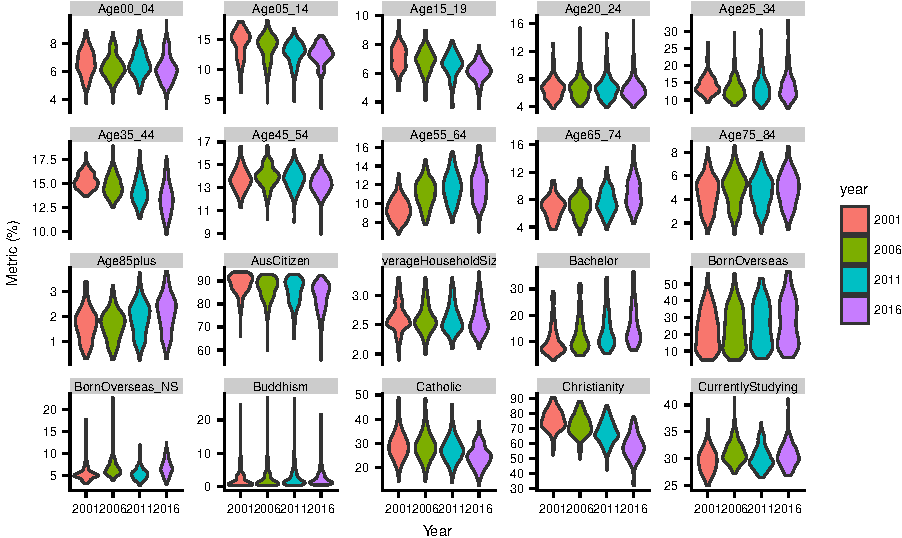
\includegraphics{thesis_files/figure-latex/vis-census-1.pdf}
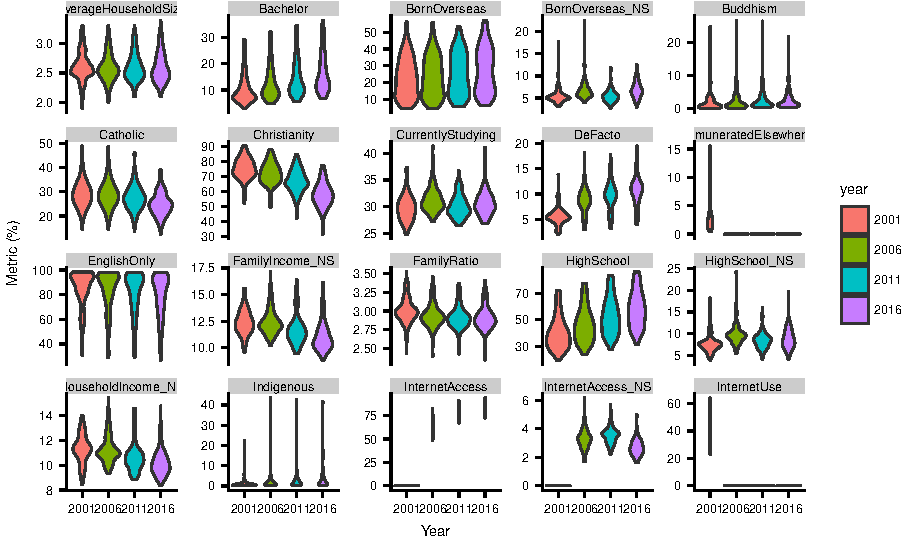
\includegraphics{thesis_files/figure-latex/vis-census-2.pdf}
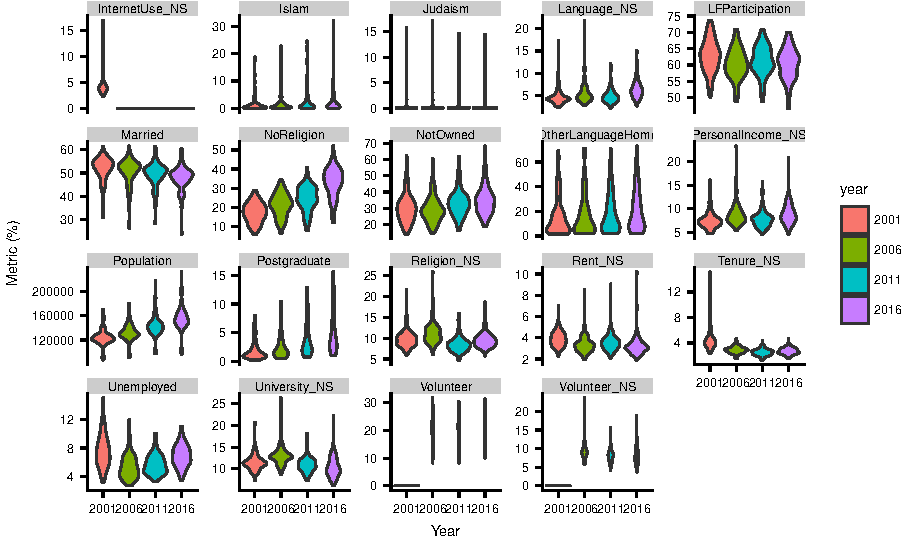
\includegraphics{thesis_files/figure-latex/vis-census-3.pdf}
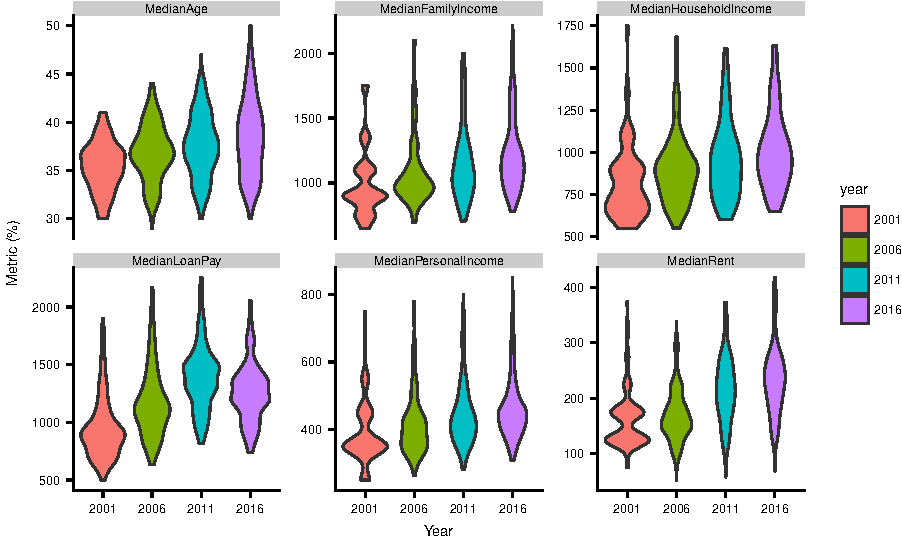
\includegraphics{thesis_files/figure-latex/vis-census-4.pdf}

\chapter{Transformation methods for logratio
analysis}\label{transformation-methods-for-logratio-analysis}

\subsection{Additive Logratio}\label{additive-logratio}

Maps to \(\mathbb{R}^{D} \text{ for } {\bf v}_i \to {\bf w}_i\)

\[\text{alr}(v_{ij}) = w_{ij} = \text{ln}(v_{ij}/v_{iD}), \space \forall \space j \in \{1,...,D\}\]

\[\text{alr}({\bf v}_i) = (\frac{\text{ln}(v_{i1})}{\text{ln}(v_{iD})}, ..., \frac{\text{ln}(v_{i(D-1)})}{\text{ln}(v_{iD})}, 1) = \text{ln}({\bf v}_i)\space \begin{bmatrix}
    1 & 0 & ... & 0 \\
    0 & 1 & ... & 0 \\
    \vdots & \vdots & \ddots & \vdots \\
    0 & 0 & ... & 1 \\
    -1 & -1 & ... & -1
\end{bmatrix}\]

Transform back to \(\textbf{v}_i\) using:
\(\textbf{v}_i = \exp(\textbf{w}_i) \cdot v_{iD}\)

\subsection{Centred Logratio}\label{centred-logratio}

Maps to \(\mathbb{R}^{D} \text{ for } {\bf v}_i \to {\bf w}_i\). Let
\(g({\bf v_i}) = \sqrt[D]{\prod_{j=1}^D v_{ij}}\).

\[\text{clr}(v_{ij}) = w_{ij} = \text{ln}(\frac{v_{ij}}{g({\bf v_i})}), \forall \space j \in \{1,...,D\}\]

\[\text{clr}({\bf v}_i) = \Big(\text{ln}(\frac{v_{i1}}{g({\bf v_i})}),...,\text{ln}(\frac{v_{iD}}{g({\bf v_i})}))\Big) \\ = \frac{\text{ln}({\bf x}_i)}{D} \cdot \begin{bmatrix}
    D-1 & -1 & ... & -1 \\
    -1 & D-1 & ... & -1 \\
    \vdots & \vdots & \ddots & \vdots \\
    -1 & -1 & ... & D-1
\end{bmatrix}\]

Transform back to \(\textbf{v}_i\) using:
\(v_{ij} = \frac{\exp(w_{ij})}{\sum_{j=1}^D \exp(w_{ij})}\)

\subsection{Isometric Logratio}\label{isometric-logratio}

Maps to \(\mathbb{R}^{D-1} \text{ for } {\bf v}_i \to {\bf w}_i\).

\[\text{ilr}_M({\bf v}_i) = clr({\bf v}_i)\cdot{\bf M} = \text{ln}({\bf v}_i) \cdot {\bf M}\]

Where \(\bf M\) is a matrix of \(D\) rows and \(D-1\) columns such that
\({\bf M} \cdot {\bf M}^t = {\bf I}_{D-1}\). \({\bf I}_{D-1}\) is the
identity matrix of \(D-1\) elements.

Transform back to \(\bf{v}_i\) as:
\({\bf v}_i = \exp({\bf w}_i \space \cdot \space {\bf M^{-1}})\)

\chapter{Raw ABS Census data
snapshot}\label{raw-abs-census-data-snapshot}

\begin{figure}

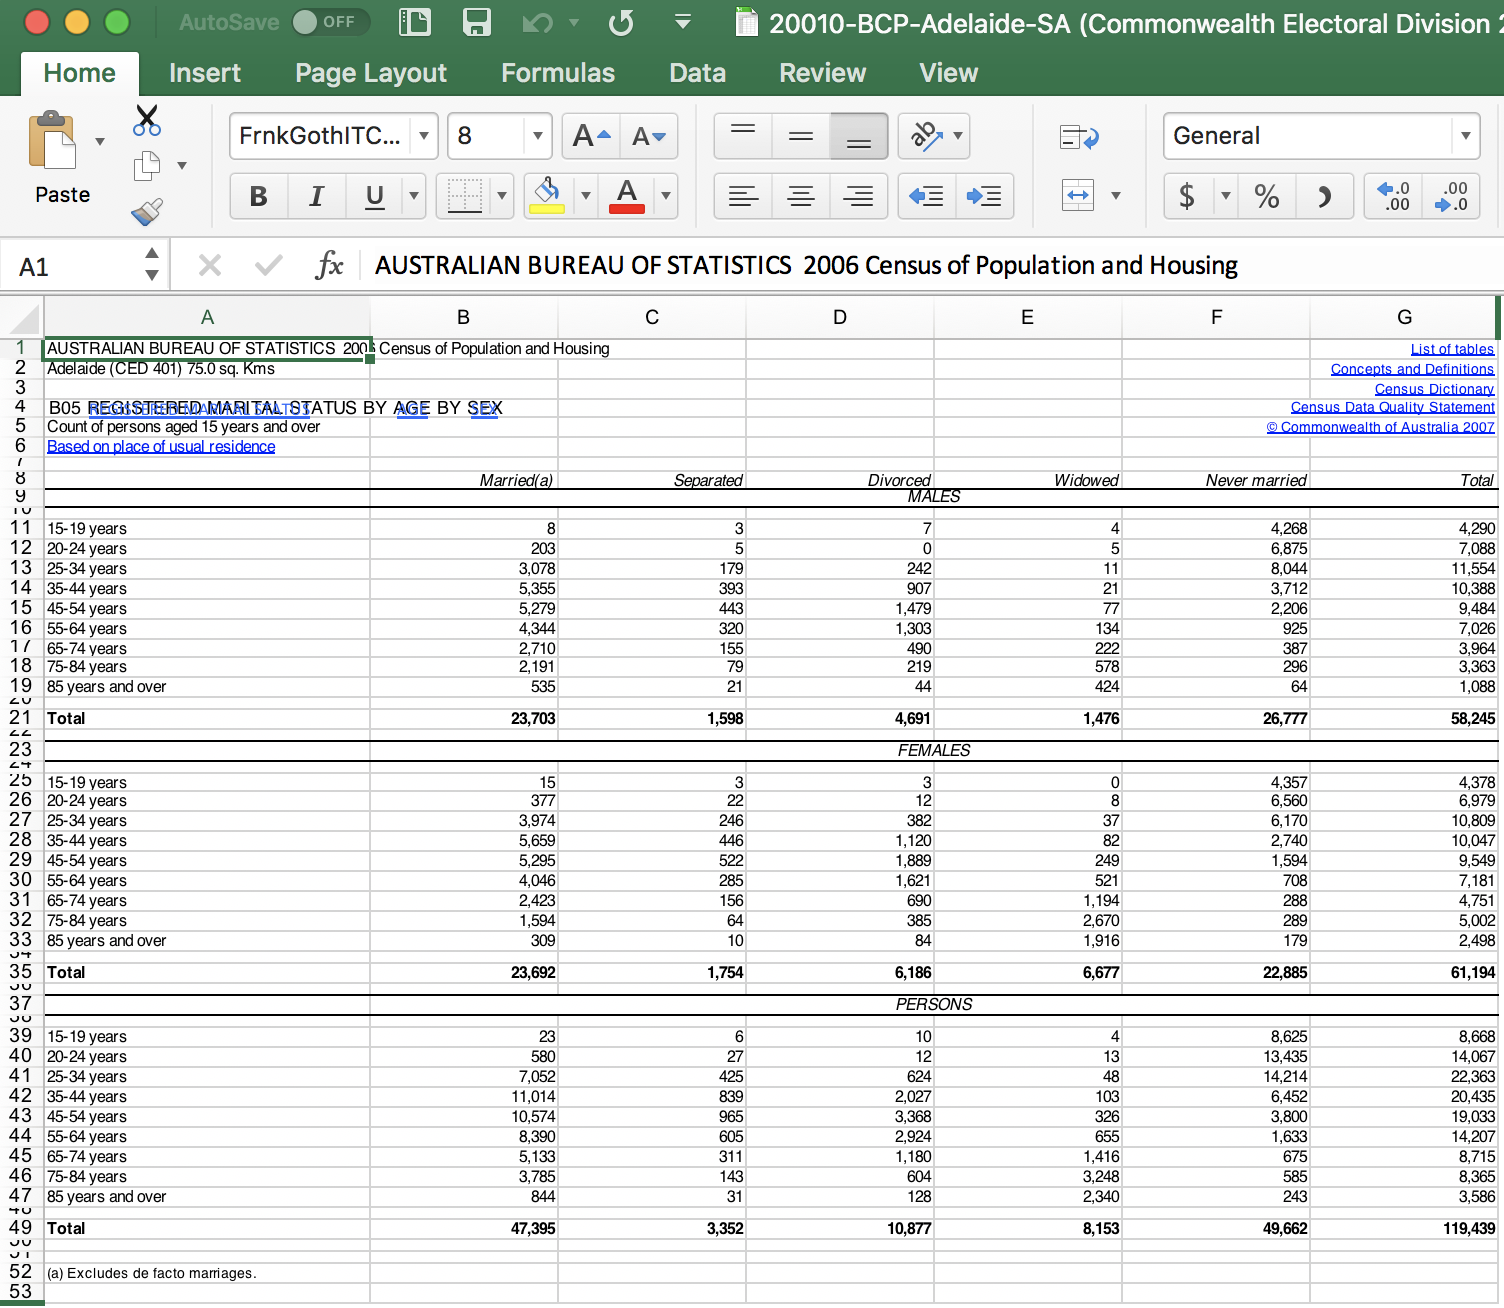
\includegraphics[width=0.8\linewidth]{/Users/Jeremy/Documents/R/MonashThesis-master-DONOTEDIT/figures/excel-screenshot} \hfill{}

\caption{Screenshot of excel document containing responses to a question from the 2004 Census}\label{fig:excel-demo}
\end{figure}

\printbibliography[heading=bibintoc]



\end{document}
